\documentclass{include/protokollclass}
% Main File - Based on protokollclass.cls
% Comments are mostly in English (and some in German, concerning the Praktikum)
% ------------------------------------------------------------------------------
% Further files in folder:
%  - include/cmds.tex (for macros and additional commands)
%  - include/kitlogo.pdf (for titlepage)
%  - lit.bib (bibtex bibliography database)
%  - include/titlepage.tex (for layout of titelpage)
% ------------------------------------------------------------------------------
% Useful Supplied Packages:
% amsmath, amssymb, mathtools, bbm, upgreek, nicefrac,
% siunitx, varioref, booktabs, graphicx, tikz, multicol

\usepackage{rotating}
\usepackage{icomma}
\usepackage{subfig}
\usepackage{pdfpages}
\usepackage[onehalfspacing]{setspace}


%% ---------------------------------------------
%% |    Informationen über dieses Protokoll    |
%% ---------------------------------------------
\newcommand{\praktikum}{P1}                % P1 oder P2
\newcommand{\semester}{WS16/17}            % z.B. "WS14/15" oder "SS15"

\newcommand{\wochentag}{Di}                % Mo, Di, Mi oder Do
\newcommand{\gruppennr}{04}                % Zweistellige Gruppennummer

\newcommand{\nachnamea}{Friedrich}             % Nachname des ersten Praktikanten
\newcommand{\vornamea}{Tabea}               % Vorname des ersten Praktikanten
\newcommand{\nachnameb}{Stockmeier}              % Nachname des zweiten Praktikanten
\newcommand{\vornameb}{Lea}              % Vorname des zweiten Praktikanten

\newcommand{\emailadressen}{lea.stockmeier@web.de, tabea.friedrich@t-online.de}
% optionale Angabe von Emailadresse(n) für den Kontakt mit dem Betreuer

\newcommand{\versuch}{Geoelektrik} % Name des Versuchs
\newcommand{\versuchsnr}{80}               % bitte die korrekte Nummer dem 
                                           % Arbeitsplatz am Versuchstag 
                                           % entnehmen
\newcommand{\fehlerrechnung}{Nein}         % Ob Fehlerrechnung im Versuch 
                                           % durchgeführt wurde oder nicht

\newcommand{\betreuer}{M. Mustermann}      % Name des zuständigen Betreuers
\newcommand{\durchgefuehrt}{01.09.16}      % Datum, an dem der Versuch 
                                           % durchgeführt wurde





%% --------------------------------------
%% |    Settings for Word Separation    |
%% --------------------------------------
% Help for separation:
% In German package the following hints are additionally available:
% "- = Additional separation
% "| = Suppress ligation and possible separation (e.g. Schaf"|fell)
% "~ = Hyphenation without separation (e.g. bergauf und "~ab)
% "= = Hyphenation with separation before and after
% "" = Separation without a hyphenation (e.g. und/""oder)

% Describe separation hints here:
\hyphenation
{
    über-nom-me-nen an-ge-ge-be-nen
    %Pro-to-koll-in-stan-zen
    %Ma-na-ge-ment  Netz-werk-ele-men-ten
    %Netz-werk Netz-werk-re-ser-vie-rung
    %Netz-werk-adap-ter Fein-ju-stier-ung
    %Da-ten-strom-spe-zi-fi-ka-tion Pa-ket-rumpf
    %Kon-troll-in-stanz
}





% um die Titelseite per PDF-reader auszufüllen. Vorgefertigte Daten
% können in Datei 'data.tex' modifiziert werden.
%\setboolean{forminput}{true}
% um die Anmerkungen zu den Textfeldern anzeigen zu lassen
%\setboolean{showannotations}{true}
% Erneuern der Seitenzahl in jedem Kapitel
%\setboolean{chapResetPageNumb}{true}
% Einbinden der Kapitelnummer in der Seitenzahl
%\setboolean{chapWiseNumb}{true}
% english or ngerman (new german für neue deutsche Rechtschreibung statt german)
\SelectLanguage{ngerman}

\title{Geophysikalische Geländeübungen \\ SS 2018 \\ Geoelektrik}
\subtitle{Messgebiet A59/1 (Riedheim)}
\author{\\ Svenja Müller \\ mueller-svenja@gmx.net
\\ \\und\\ \\
Lea Stockmeier \\ lea.stockmeier@web.de \\ \\ \\
Betreuer: Vorname1 Nachname1 und Vorname2 Nachname2}
\date{\vfill\vfill\vfill \today}


%% -----------------------
%% |    Main Document    |
%% -----------------------
\begin{document}
    % Titlepage und ToC
    \FrontMatter

    \maketitle

    \begingroup \let\clearpage\relax    % in order to avoid listoffigures and
    \tableofcontents                    % listoftables on new pages
    \listoffigures
    \listoftables
    \endgroup
    %\cleardoublepage



    % Contents
    \MainMatter
    
%     \emptychapter[1]{Messprotokoll 1}{} % usage: \emptychapter[page displayed 
                                        %        in toc]{name of the chapter}
%     \pseudochapter[3]{Messprotokoll 2}  % usage: \pseudochapter[number of pages 
                                        %        added]{name of the chapter}
    
    \chapter{Einleitung}
    Bei der geophysikalischen Geländeübung 2018 führten wir am ersten Messtag, den 22.05., die Magnetik-Messungen durch. Das folgende Protokoll beschreibt die Theorie, Versuchsdurchführung, Auswertung und Fehlerdiskussion zu diesem Versuch.

Bei den Messungen und im Protokoll verfolgten wir folgende Fragestellungen: Die erste große Fragestellung ist, ob mit der Magnetik der Gang lokalisiert werden kann. Bei der Kartierung stellten wir uns die Frage, ob wir den Gang so gut lokalisieren können, dass wir uns daran die Lage der weiteren Profile überlegen können.
Bei den Profilen stellten wir uns dann die Frage, ob diese wirklich senkrecht zum Gang angelegt wurden. Dazu dient vor allem ein Profil, das extra schräg zum Gang gewählt wurde, um zu sehen, ob überhaupt ein Unterschied festgestellt werden kann. Die senkrechten Profile sollen zeigen, ob ein gemeinsames, alle Verläufe der Totalintensitäten erklärendes Modell gefunden werden kann. Die Messungen mit dem Fluxgate verfolgen die Fragestellung, ob dabei sinnvoll das Zweikreisverfahren angewendet werden kann. Die Vermessung eines vorbeifahrenden Traktors und der Umgebung der Basisstation dienten zur Abschätzung der während der Messung durch äußere Einflüsse auftretenden Fehler.
    
    \chapter{Theoretische Grundlagen}
    
Mit geoelektrischen Messungen werden Materialeigenschaften wie die Ionenkonzentration, Grad der Wassersättigung und der Permeabilität untersucht. 
Das bedeutet dass mit Hilfe dieses Verfahrens z.B der Grundwasserspiegel bestimmt werden kann. \\
Bei den Messmethoden wird zwischen aktiven und passiven Verfahren unterschieden.  Da sowohl bei der Schlumberger-Sondierung als auch bei der Wenner-Karitierung wir eine Spannung angelegt, wodurch die beiden Verfahren zu den aktiven Messmethoden gezählt werden.



Während der Geländeübung werden die Messungen mit dem Wechselstromverfahren durchgeführt. Dabei wird an zwei Elektroden Wechselstrom angelegt,
über zwei Sonden an der Oberfläche wird die Spannung gemessen. Mit diesem Verfahren wird also die Materialeigenschaft elektrischen Strom zu leiten untersucht. \\
Hierbei unterscheidet man zwischen elektrischer Leitfähigkeit, wenn Elektronen bewegt werden, und ionischer Leitfähigkeit, dem Transport von Ionen. 
Aufgrund der elektrischen Leitfähigkeit können z.B Metallrohre im Boden lokalisiert werden. Ionische Leitfähigkeit tritt in Gesteinen und Lockersedimenten auf,die einen entsprechenden Wassergehalt haben. \\
\\
Als Materialeigenschaft wird der spezifischen Widerstands $$[\rho] = \SI{1}{\Omega m}$$ bestimmt, er ist der Kehrwert der Leitfähigkeit $\sigma$. Je nach Material und Wassergehalt variieren diese Werte. Es wird eine ein Strom in die Erden eingespeist und Anhand des Spannungsabfalls, der mit Hilfe der Sonden gemessen wird, wird auf den Wiederstand der Stromdurchflossenen Materalien geschlossen. Während der Geländeübung wird ein Basaltgang untersucht. Basalt hat einen relativ hohen spezifischen Widerstand, so das er durch ein Ansteigen  von $ \rho$ lokalisiert werden kann.

\section{Schlumberger-Anordnung}
Die Schlumberger-Anordnung wird in der Geländeübung zur Sondierung verwendet. Es wird die Änderung des spezifischen Widerstands in den verschiedenen Schichten den Untergrunds unter einem bestimmten Punkt bestimmt. In Abbildung \ref{abb:Schlumberger} ist die Schlumberger-Anordung schematisch dargestellt. Der Ort an dem gemessen wird ist der Mittelpunkt der Anordnung. Um in verschieden Tiefen Messwerte zu erhalten wird der Anstand zwischen den Elektroden und den Sonden jeweils symmetrisch erhöht. Sinnvoll ist es den Abstand exponentiell zu erhöhen und ein Profil mit möglichst wenig Topographie zu wählen.\\
Beim Stecken der Stromelektroden ist es wichtig eine möglichst große Kontaktfläche zu haben, da es an diesen zu Kontaktwiderstand kommt. Eine große Kontaktfläche erreicht man indem man die Stromelektroden möglichst tief in die Erde steckt. 
Das gleiche gilt natürlich für die Wenner-Kartierung.


%%%%%%%%%%%%%%%%%%%%%%%%%%%%%%%%%%%%%
\begin{figure}[h]
\centering
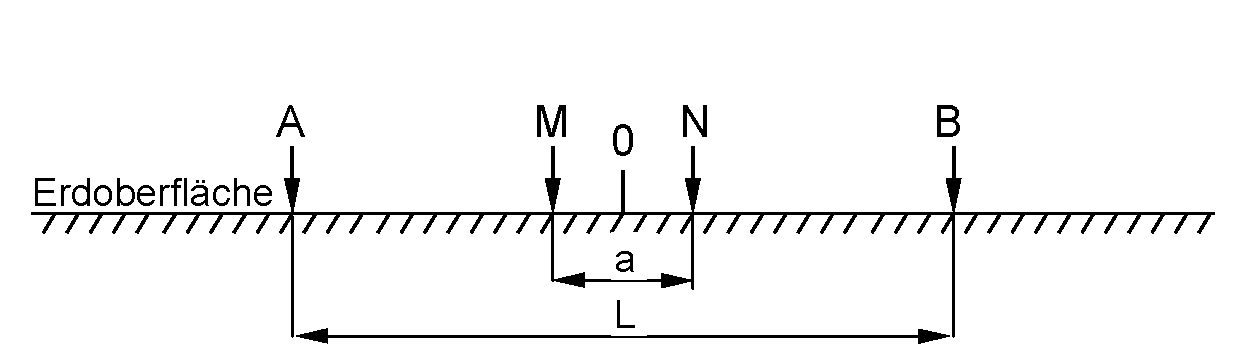
\includegraphics[width=0.6\textwidth]{Schlumberger.png}
\caption{Schematische Darstellung der Schlumberger-Anordnung}
\label{abb:Schlumberger}
\end{figure}
%%%%%%%%%%%%%%%%%%%%%%%%%%%%%%%%%%%%

\section{Wenner-Kartierung}
In Abbildung \ref{abb:Wenner} ist der schematische Aufbau der Wenner-Anordnung zu sehen. Bei \textbf{A} und \textbf{B} sind die Elektroden und bei \textbf{M}, \textbf{N} die Sonden zur Spannungsmessung.

%%%%%%%%%%%%%%%%%%%%%%%%%%%%%%%%%%%%%
\begin{figure}[h]
\centering
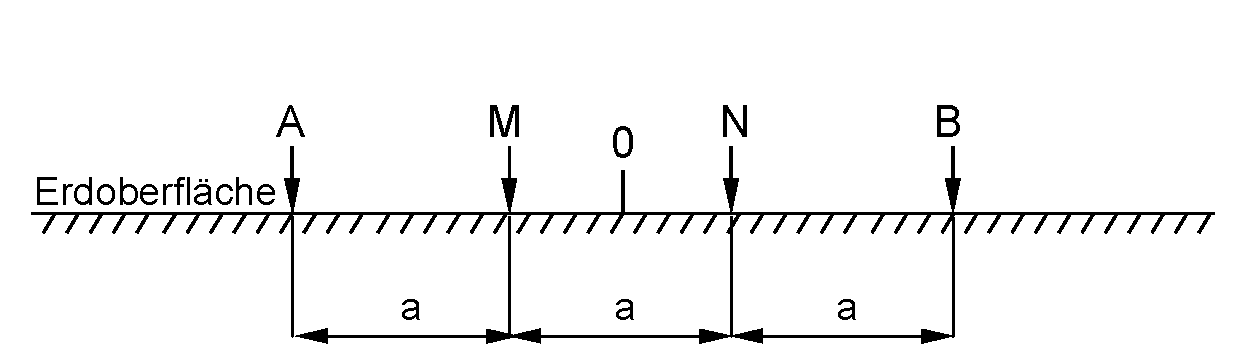
\includegraphics[width=0.6\textwidth]{Wenner.png}
\caption{Schematische Darstellung der Schlumberger-Anordnung}
\label{abb:Wenner}
\end{figure}
%%%%%%%%%%%%%%%%%%%%%%%%%%%%%%%%%%%%

Bei der Wenner-Kartierung werden die Abstände zwischen den Elektroden konstant gehalten und die ganze Anordnung wird über den Boden verschoben. Somit wird in einer Tiefe an verschieden, horizontal versetzten, Punkten im Untergrund gemessen. Der Abstand $a$ der Elektroden entspricht auch der Tiefe in der die Messung durchgeführt wird. \\
Hierbei muss aber bedacht werden, dass oben leigende, sehr gut leitende Schichten den Strom bündeln kann und somit zu einem verfälschten Messergebnis führen können.

\section{Geoelektrische Tomographie}
Die Tomographie ist eine Mischung aus der Wenner-Karierung und Schlumberger-Sondierung. Die Wenner-Karierung wird praktisch in verschiedenen Tiefen durchgeführt und über eine Profil bewegt, dadurch wird ein zweidimensionales Bild des Untergrunds erstellt.
Mit Hilfe eines Comuterprogramms kann durch Inversion der gemessenen Werte ein Modell für die Verteilung des spezifischen Widerstands im Untergrund erstellt werden.



\section{Spezifischer Widerstand und Geometriefaktor}

Die Potentialdifferenz bei einem Angelegten Strom I ist
\begin{equation}
V = \rho \, I \, \frac{1}{2 \pi} \big(\frac{1}{r_{\mathrm{AM}}} - \frac{1}{r_{\mathrm{MB}}} + \frac{1}{r_{\mathrm{NB}}} - \frac{1}{r_{\mathrm{AN}}} \big) \, ,
\end{equation}
wobei mit $r_{\mathrm{AM}}$ usw. jeweils die Abstände zwischen den Sonden und Elektroden, wie in Abbildung \ref{abb:Wenner} zu sehen, bezeichnet werden.
Um den spezifischen Widerstand leichter berechnen zu können wird der Geometriefaktor $F$ eingeführt,
$$F = \frac{2 \pi}{\frac{1}{r_{\mathrm{AM}}} - \frac{1}{r_{\mathrm{MB}}} + \frac{1}{r_{\mathrm{NB}}} - \frac{1}{r_{\mathrm{AN}}}}\,.$$
Damit lässt sich $\rho$ berechnen mit 
\begin{equation}
\rho = \frac{V}{I} \, F.
\end{equation} \label{eq:roh}

\textbf{Scheinbarer spezifischer Widerstand}

Ist der Untergrund nicht homogen, dann wird der Wert der Formel \ref{eq:roh} als scheinbarer spezifischer Widerstand bezeichnet. Der Geometriefaktor hängt nur von der geometrischen Anordnung ab und nicht von der 
Leitfähigkeit des Untergrunds, weshalb der scheinbare spezifische Widerstand $q_a$ nur im Falle eines homogenen Untergrunds gleich dem spezifischen Widerstands ist.\\
Im Falle der Wenner-Anordnung wird  der scheinbare spezifische Widerstand mit der Formel
$$ \rho_a = 2 \pi \frac{V}{I} a $$
berechnet.
Bei einer Messung wird versucht durch Interpretation der gemessenen scheinbaren Widerstände den spezifischen Widerstand zu finden.












    
    \chapter{Versuchsbeschreibung}
    %Versuchsbeschreibung
In der Geoelektrik wurden drei verschiedene Messmethoden verwendet. Das sind die Wenner-Kartierung, Schlumberger-Sondierung und die Tomographie. Sowohl die Wenner-Kartierung als auch die Tomographie wurde über dem Basaltgang durchgeführt, um diese Messmethode mit den übrigen vergleichen zu können.

In Abbildung \ref{abb:PBasalt} sind die Profile der Wenner-Kartierung und Tomographie abgebildet. Die Wenner-Kartierung wurde entlang E11-E12 durchgeführt und das Profil der Tomographie ist in dieser Abbildung beschriftet. Zu sehen ist, dass das Profil der Geoelektrik über dem Profil der Magnetik und Gravimetrie liegt. Dadurch kann man direkt die Messergebnisse vergleichen und eventuell sehen, welche Methode sich zum Untersuchen des Basalts eignet und welche nicht.

Die Schlumberger-Sondierung wurde auf dem gleichen Profil wie die Seismik-Messung mit Sissy durchgeführt, um die beiden Messungen vergleichen zu können. Dieses Profil ist das obere Profil E21-E22 in Abbildung \ref{abb:PWiese}.

%%%%%%%%%%%%%%%%%%%%%%%%%%%%%%%%%%%%%
\begin{figure}[ht]
\centering
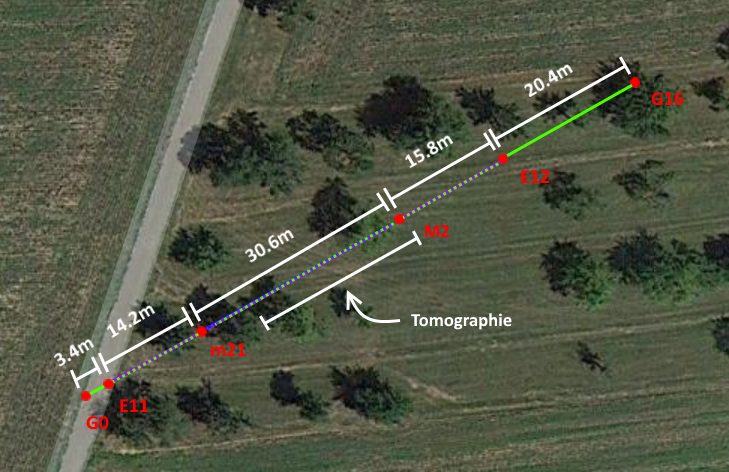
\includegraphics[width=0.6\textwidth]{fig/ElektrikMagnetikGravimetrie0gps.png}
\caption[Profile der Geoelektrik, Gravimetrie und Magnetik des Messgebiets am Basaltgang]{Profile der Geoelektrik, Gravimetrie und Magnetik des Messgebiets am Basaltgang. Die Graphik wurde von Rebekka Kirchgässner und Luisa Rank übernommen.}
\label{abb:PBasalt}
\end{figure}
%%%%%%%%%%%%%%%%%%%%%%%%%%%%%%%%%%%%

%%%%%%%%%%%%%%%%%%%%%%%%%%%%%%%%%%%%%
\begin{figure}[ht]
\centering
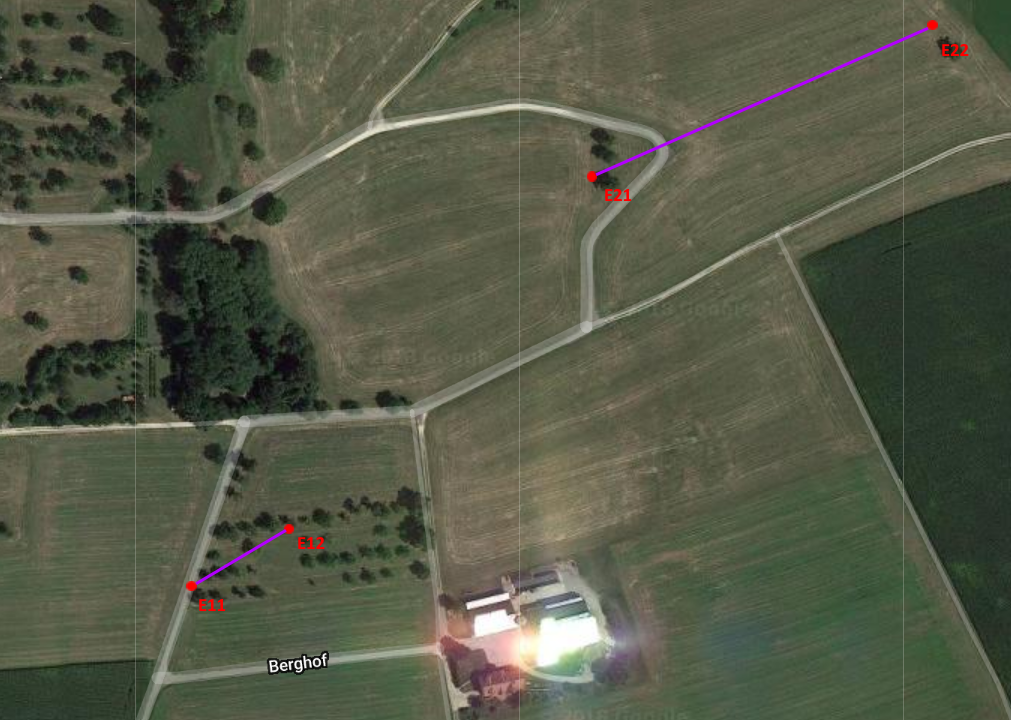
\includegraphics[width=0.6\textwidth]{fig/profilegps.PNG}
\caption[Profil E11-E12 und E21-E22 auf den beiden Messgebieten]{Profil E11-E12 und E21-E22 auf den beiden Messgebieten. Die Graphik wurde von Rebekka Kirchgässner und Luisa Rank übernommen.}
\label{abb:PWiese}
\end{figure}
%%%%%%%%%%%%%%%%%%%%%%%%%%%%%%%%%%%%
\newpage

\section{Wenner-Katierung}

Begonnen wurde mit der Wenner-Kartierung, um die Lage des Basaltgangs genauer zu bestimmen. Damit wir die Tomographie möglichst genau über dem Gang durchführen
können. 
Des weiteren soll eingeschätzt werden, wie gut diese Methode zum Vermessen des Basaltgangs geeignet ist.

Die Kartierung wurde in einer Tiefe von 5\,m vorgenommen. Dies ist begründet mit der Annahme, dass der Basaltgang vermutlich in ca. 1-2\,m Tiefe beginnt und nach unten 
als unendlich angenommen werden kann. Je mehr Basalt im Bereich der Messung ist, desto größer ist die Auswirkung auf die Ergebnisse.
Die Anordnung ist orthogonal zum Basaltgang und wird auch orthogonal dazu verschoben. Orientiert wurde sich dabei an der Messung von Magnetik, es wurde 
entlang des Magnetik-Profils M2-M21 gemessen. Dabei wurde darauf geachtet, dass auch eine Messung komplett außerhalb 
des Einflussbereichs des Basalt liegt.

\section{Tomographie}

Die Tomographie ist eine Kombination der ersten beiden Messmethoden. Sie wurde auf dem gleichen Profil wie die Wenner-Kartierung durchgeführt.
Es wurden 48 Elektroden verwendet, die in einem Abstand von 50\,cm, auf der gleichen Messlinie wie bei der Wenner-Kartierung aufgestellt waren. 
Die Mitte der Messlinie wurde auf einen Punkt gesetzt, an dem auch die Mitte des Basaltgangs vermutet wurde. Insgesamt wurde also auf einer Länge von 24\,m gemessen.
Als 0-Punkt für die Messung wurde das obere Ende des Messbands festgelegt.
Nachdem die Elektroden aufgestellt und angeschlossen wurden, wurde die Messung automatisch mit einem Messgerät ausgeführt. Auf das Ergebnis musste ungefähr 
eine Stunde gewartet werden. Das Messprotokoll zur Tomographie befindet sich im Anhang unter der Abbildung \ref{abb:AnhTomographie}.

\section{Schlumberger-Sondierung}

Sie Schlumberger-Sondierung wurde nicht auf dem Messgebiet über dem Basaltgang vorgenommen, sondern auf einer Wiese wesentlich weiter oben. Auf dieser Wiese wurde 
bereits mit der Seismik gemessen. Um unsere Ergebnisse von der Seismik-Messung und dieser Messung vergleichen zu können, wurde die Messung entlang der gleichen
Linie durchgeführt.

Da wir kein sehr großes, gerades Gelände hatten und auch mit der Seismik in keinen großen Tiefen gemessen wurde, betrug die Länge des Profils 200\,m. Als Mitte 
haben wir den Punkt des Mittelschusses der Hammerschlag-Methode (Seismik) verwendet.
In der Mitte des Profils haben wir angefangen, die Elektroden zu stecken. In beide Richtungen haben wir den Abstand exponentiell vergrößert. Die genauen Abstände kann man dem Messprotokoll dieser Messung im Anhang entnehmen.
    
    \chapter{Auswertung}
    %Auswertung
\section{Wenner-Kartierung}

Die Wenner-Kartierung wurde auf einem 46\,m langen Profil E11-E12 senkrecht zum Basaltgang durchgeführt. Die Messprotokolle dazu befinden sich im Anhang in den Abbildungen  \ref{abb:Wenner1} und \ref{abb:Wenner2}. 
Die spezifischen Widerstände wurden bereits im Feld mit Hilfe der Formel~\eqref{eq:roh} aus Kapitel~\ref{sec:spezW} berechnet.
% In Tabelle \ref{tab:wenner} sind die gemessenen Werte des spezifischen Widerstands mit dem entsprechenden festgelegten Abstand zu sehen.
% Die spezifischen Widerstände wurden mit Hilfe der Formel \eqref{eq:roh} aus Kapitel \ref{sec:spezW} und den Werten der Tabellen \ref{abb:Wenner1} und \ref{abb:Wenner2} berechnet.
Die Abstände
der Messpunkte sind in der Mitte den Profils kleiner gewählt als außen, da wir dort den Basaltgang vermuten. Aus den Messergebnissen der Magnetik-Messungen konnte schon sehr genau abgeschätzt werden, wo der Basaltgang liegt.

%%%%%%%%%%%%%%%%%%%%%%%%%%%%%%%%%%%%%%%%%%%%%%%%%%%%%%%%%%%%%%%%%%%%
% \begin{table}[!ht]
% \centering
% \caption{Messwerte der Wenner-Kartierung}
% \begin{tabular}{ c  c  | c  c}
% \toprule
% Abstand in m  & Widerstand in $\Omega$m &  Abstand in m & Widerstand in $\Omega$m \\
% \midrule
% 0    & 15.873 & 25   & 32.673 \\
% 1    & 15.605 & 25.5 & 33.126 \\
% 2    & 16.036 & 26   & 29.951 \\
% 3    & 16.431 & 26.5 & 27.679 \\
% 4    & 16.658 & 27   & 25.546 \\
% 5    & 15.33  & 27.5 & 24.013 \\
% 6    & 15.155 & 28   & 23.626 \\
% 7    & 15.029 & 28.5 & 22.262 \\
% 8    & 15.044 & 29   & 21.232 \\
% 9    & 15.765 & 29.5 & 20.754 \\
% 10   & 18.122 & 30   & 20.354 \\
% 11   & 19.323 & 30.5 & 19.708 \\
% 12   & 20.27  & 31   & 21.024 \\
% 13   & 20.403 & 31.5 & 22.026 \\
% 14   & 20.054 & 32   & 22.442 \\
% 15   & 18.457 & 32.5 & 22.334 \\
% 15.5 & 18.217 & 33   & 21.789 \\
% 16   & 17.687 & 33.5 & 22.438 \\
% 16.5 & 17.456 & 34   & 22.927 \\
% 17   & 16.948 & 34.5 & 21.875 \\
% 17.5 & 16.859 & 35   & 20.88  \\
% 18   & 17.779 & 35.5 & 21.11  \\
% 18.5 & 18.37  & 36   & 20.109 \\
% 19   & 19.392 & 36.5 & 19.245 \\
% 19.5 & 20.363 & 37   & 19.105 \\
% 20   & 21.945 & 37.5 & 18.882 \\
% 20.5 & 23     & 38   & 18.774 \\
% 21   & 25.416 & 39   & 18.104 \\
% 21.5 & 30.071 & 40   & 18.712 \\
% 22   & 25.125 & 41   & 18.659 \\
% 22.5 & 31.057 & 42   & 19.165 \\
% 23   & 31.101 & 43   & 19.466 \\
% 23.5 & 32.759 & 44   & 20.332 \\
% 24   & 33.908 & 45   & 25.904 \\
% 24.5 & 33.561 & 46   & 20.623 \\
% \bottomrule
% \end{tabular}
% \label{tab:wenner}
% \end{table}
%%%%%%%%%%%%%%%%%%%%%%%%%%%%%%%%%%%%%%%%%%%%%%%%%%%%%%%%%%%%%%%%%%%%

In Abbildung \ref{abb:Wennerdiagr} sind die Messergebnisse
% aus Tabelle \ref{tab:wenner}
graphisch dargestellt. Wir gehen davon aus, dass der Basalt eine andere Leitfähigkeit hat als das Umgebungsmaterial und sich die magnetischen Eigenschaften und elektrische Leitfähigkeit 
gleichzeitig ändern. Das ist die Voraussetzung dafür, dass wir mit Hilfe unserer Ergebnisse aus der Magnetik unser Profil für die Geoelektrik festlegen können und in beiden Versuchen ähnliche Ergebnisse erhalten.

%%%%%%%%%%%%%%%%%%%%%%%%%%%%%%%%%%%%%%%%%
\begin{figure}[ht]
\centering
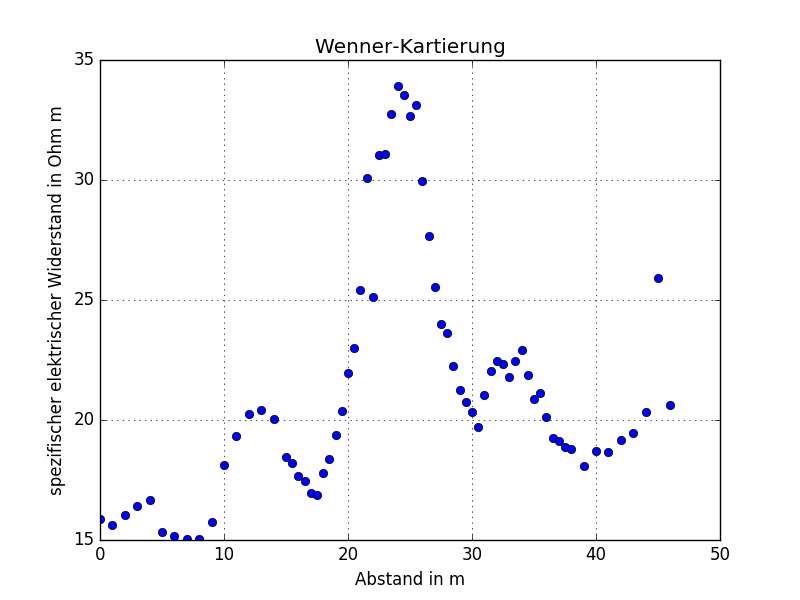
\includegraphics[width=0.8\textwidth]{fig/wennerkartierung.png}
\caption[Diagramm unserer Ergebnisse der Wenner-Kartierung]{Diagramm unserer Ergebnisse der Wenner-Kartierung. Der gemessene spezifische Widerstand ist gegen den Abstand zu unserem gewählten Null-Punkt aufgetragen. Der Null-Punkt wurde so gewählt, dass er mit dem Null-Punkt der Tomographie übereinstimmt}
\label{abb:Wennerdiagr}
\end{figure}
%%%%%%%%%%%%%%%%%%%%%%%%%%%%%%%%%%%%

Deutlich zu sehen ist ein Maximum des spezifischen Widerstands in der Mitte des Diagramms \ref{abb:Wennerdiagr}.
Dies weist darauf hin, dass der Basaltgang wie vermutet in der Mitte unseres Profils liegt.
Rechts und links des großen Maximums sind weitere kleinere Nebenmaxima zu erkennen. Da wir den Untergrund nicht genau kennen, können wir nicht mit Sicherheit sagen, um was es sich dabei handelt. Wir vermuten, dass der Basaltgang etwas verwittert 
ist, sich z.B. durch Wasser Risse im Gestein gebildet haben. Hat sich nun zwischen dem abgespalteten Basalt leitfähiges Material eingelagert, wird an diesen Stellen ein geringerer spezifischer Widerstand gemessen.
Da die Nebenmaxima nicht die gleiche Höhe haben wie das Maximum in der Mitte, ist es auch wahrscheinlich, dass der Basaltgang nicht nur durch Risse unterteilt ist. Wir gehen davon aus, dass der Basalt an den Rändern sehr stank verwittert ist.
Grob stimmen unsere Erkenntnisse mit denen der Magnetik überein.
%Grob genauer!!??? Was stimmt überein?

\section{Tomographie}

In Abbildung \ref{abb:Tomographie} sind die Ergebnisse der Tomographie-Messung zu sehen. Die obere Abbildung zeigt die von uns gemessenen Werte für den scheinbaren spezifischen Widerstand. Die Inversion der Werte, also ein Modell wie der Untergrund 
wirklich aussehen könnte, ist im unteren Diagramm zu sehen. In der Mitte ist dargestellt, welche Widerstandswerte man gemessen hätte, wenn der Untergrund dem berechneten Modell entsprechen würde.
Die beiden oberen Diagramme sind nahezu identisch, also sehr ähnlich. Das bedeutet dass, das berechnete Modell unsere gemessenen Werte sehr gut beschreibt.

%%%%%%%%%%%%%%%%%%%%%%%%%%%%%%%%%%%%
\begin{figure}[ht]
\centering
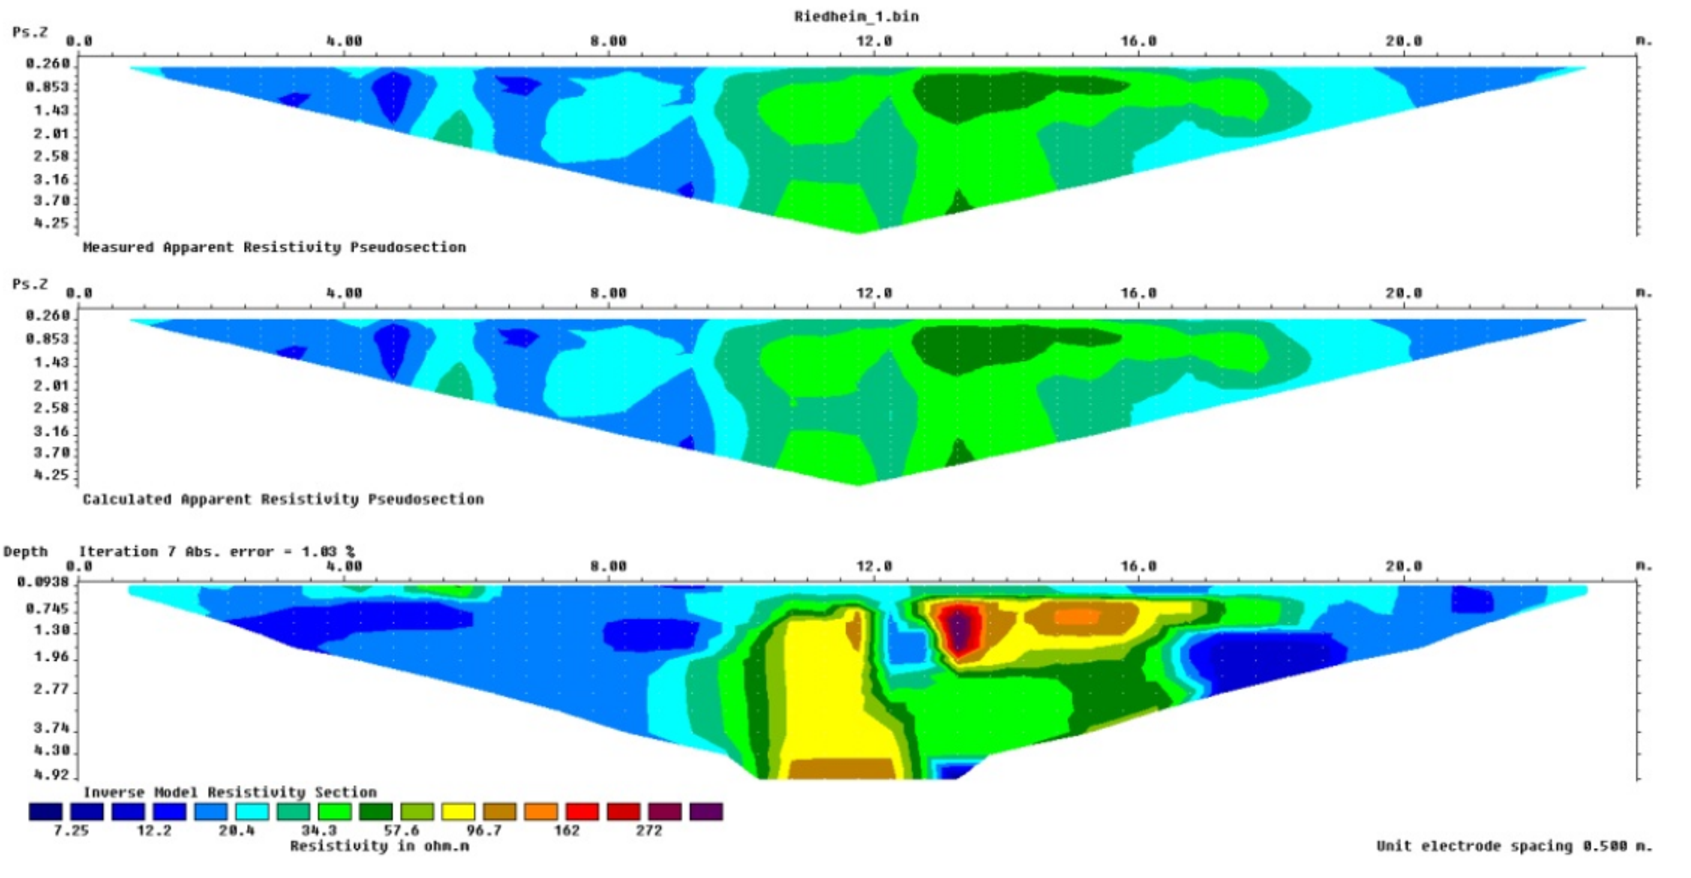
\includegraphics[width=\textwidth]{fig/Tomographie.pdf}
\caption[Tomographie-Modell]{Tomographie-Modell. Als Anfangspunkt der Messung wurde das obere Ende der Profillinie gewählt.}
\label{abb:Tomographie}
\end{figure}
%%%%%%%%%%%%%%%%%%%%%%%%%%%%%%%%%%%%

Bei dem Abstand 13\,m ist eine sehr starke Anomalie von ca. $ \SI{300}{\Omega m}$. Die Anomalie ist jedoch sehr klein und oberflächennah. Links davon ist eine zweite, sehr deutliche Anomalie zu sehen, die in dem gemessenen Bereich
mit zunehmender Tiefe größer wird. Der spezifische Widerstand ist hier aber nur maximal etwa $\SI{100}{\Omega m}$.
Etwa $\SI{2}{m}$ entfernt von der stärksten Anomalie, bei  $\SI{14}{m}$ beginnt eine dritte, oberflächennahe Anomalie.

Beim Vergleich mit den Ergebnissen der Wenner-Kartierung finden wir große Ähnlichkeiten. Die Tomographie deutet, ebenso wie die Wenner-Kartierung, darauf hin, dass der Basaltgang an der gemessenen Stelle grob in drei Teile unterteilt werden kann. Dies könnte von Karstverwitterung verursacht werden.

Allerdings sollte hier noch beachtet werden, dass die Wenner-Kartierung in einer Tiefe von $\SI{5}{m}$ vorgenommen wurde. Die Tomographie an ihrem tiefsten Punkt aber nur $\SI{5}{m}$ in die Tiefe geht. 

Zunächst wurde vermutet, dass die starke Anomalie dem globalen Maximum der Wenner-Kartierung entspricht. In der Tomographie sehen wir aber, dass die Differenz dieser stärksten Anomalie und den Nebenmaxima fast $\SI{200}{\Omega m}$ beträgt, was bei einer Skala von $\SI{0}{\Omega m}- \SI{300}{\Omega m}$ sehr viel ist. Wir haben vermutet, das diese Anomalie trotz der geringen Höhe die Tomographie beeinflusst.

Diese Annahme wurde überprüft, indem wir die Ortsangaben der beiden Diagramme verglichen haben. Leider passt die Wenner-Kartierung hier nicht mehr gut zur Tomographie. Vermutlich haben die Anomalien in den oberen Schichten wirklich kaum Einfluss auf die Wenner-Kartierung. Da wir diese in 5\,m Tiefe durchgeführt haben und das Tomographie-Modell eben hier aufhört, können wir die beiden Methoden eigentlich nicht vergleichen. Was aber auch ein interessantes Ergebnis ist, da wir nun sehen, dass die Messwerte der Wenner-Kartierung wirklich nahezu nur den spezifischen Widerstand in $\SI{5}{m}$ Tiefe wiedergeben.

\section{Sondierung}

Die Sondierung wurde auf dem Profil E21-E22 durchgeführt. Die Messwerte sind in Abbildung \ref{abb:Schlumberger1} und \ref{abb:Schlumberger2} im Anhang zu sehen. Aus ihnen werden mit Hilfe des Inversionsprogramms Ipi2win Modelle für die Schichten im Untergrund erstellt.
In Abbildung \ref{abb:Schlum1} und \ref{abb:Schlum2} sind die Ergebnisse zu sehen. Die schwarze Kurve ist die Fitkurve durch unsere Messpunkte und in blau ist das Modell des spezifische Widerstands des Untergrunds dargestellt. Die rote Kurve ist der scheinbare spezifische Widerstand, der sich aus diesem Modell ergibt.

\subsection{Modell mit drei Schichten}

Als erstes haben wir ein möglichst genaues Modell erstellt mit der Annahme, dass wir drei Schichten gegeben haben. Es müssen mindestens drei Schichten sein, da die schwarze Kurve in Abbildung \ref{abb:Schlum1} am linken Ende nach unten geht. Das Ergebnis ist in Abbildung \ref{abb:Schlum1} zu sehen. Der Fehler dieses Models lag bei unter 2\%. In Abbildung \ref{abb:SchlumTab1} ist die dazugehörige Tabelle mit dem berechneten spezifischen Widerstand $\rho$, der Dicke $h$ und Tiefe $d$ der jeweiligen Schichten.  Alle drei Werte nehmen mit der Tiefe zu, was sehr plausibel ist. Die erste Schichtgrenze ist in etwa $\SI{5}{cm}$ Tiefe und die zweite schon bei $\SI{43}{cm}$, die dritte erst bei etwa $\SI{8}{m}$. Diese Ergebnisse lassen sich leider nicht mit denen der Seismik vergleichen. 

%%%%%%%%%%%%%%%%%%%%%%%%%%%%%%%%%%%%
\begin{figure}[ht]
\centering
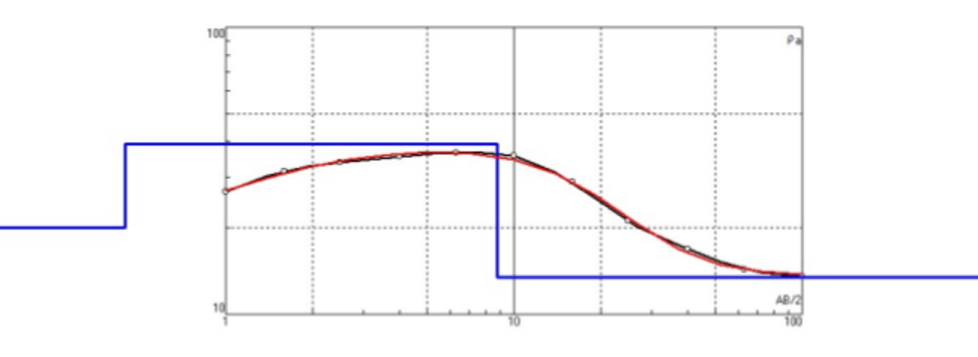
\includegraphics[width=0.8\textwidth]{fig/Schlumberger_3Schichten.pdf}
\caption{Inversionsmodel mit drei Schichten }
\label{abb:Schlum1}
\end{figure}
%%%%%%%%%%%%%%%%%%%%%%%%%%%%%%%%%%%%
%%%%%%%%%%%%%%%%%%%%%%%%%%%%%%%%%%%%
\begin{figure}[ht]
\centering
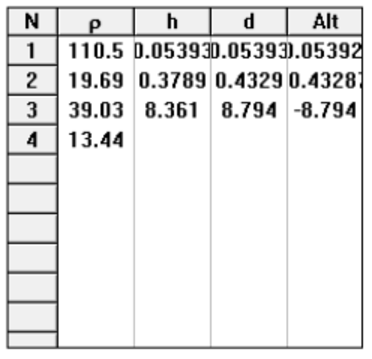
\includegraphics[width=0.3\textwidth]{fig/schlumbergerTabelle.pdf}
\caption[Daten zum Inversionsmodell mit drei Schichten]{Daten zum Inversionsmodell mit drei Schichten. $\rho$ bezeichnet den spezifischen Widerstand in $\Omega$m, $h$ die Schichtdicke in m, $d$ die Schichttiefe in~m}
\label{abb:SchlumTab1}
\end{figure}
%%%%%%%%%%%%%%%%%%%%%%%%%%%%%%%%%%%%

\subsection{Modell mir fünf Schichten}

Als zweites haben wir die Inversion ohne vorgegebene Maximalzahl der Schichten gemacht. Dabei wurde ein Modell mit 5 Schichten berechnet, welches in Abbildung \ref{abb:Schlum2} zu sehen ist. Die Tabelle mit den entsprechenden Werten ist in Abbildung \ref{abb:SchlumTab2} gegeben.

%%%%%%%%%%%%%%%%%%%%%%%%%%%%%%%%%%%%
\begin{figure}[ht]
\centering
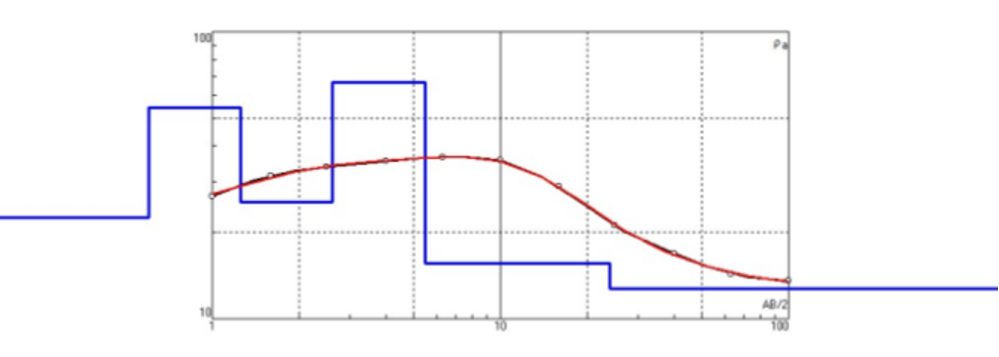
\includegraphics[width=0.8\textwidth]{fig/Schlumberger_5Schichten.pdf}
\caption{Inversionsmodell mit fünf Schichten}
\label{abb:Schlum2}
\end{figure}
%%%%%%%%%%%%%%%%%%%%%%%%%%%%%%%%%%%%
%%%%%%%%%%%%%%%%%%%%%%%%%%%%%%%%%%%%
\begin{figure}[ht]
\centering
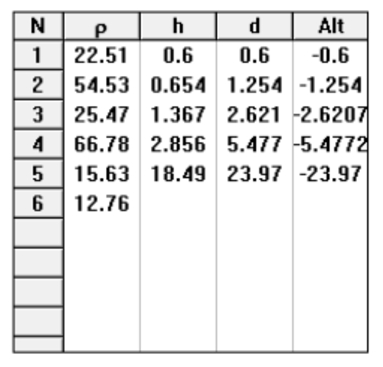
\includegraphics[width=0.3\textwidth]{fig/schlumbergerTabelle2.pdf}
\caption[Daten zum Inversionsmodell mit fünf Schichten]{Daten zum Inversionsmodell mit fünf Schichten. $\rho$ bezeichnet den spezifischen Widerstand in $\Omega$m, $h$ die Schichtdicke in m, $d$ die Schichttiefe in~m}
\label{abb:SchlumTab2}
\end{figure}
%%%%%%%%%%%%%%%%%%%%%%%%%%%%%%%%%%%%

Die erste Schichtgrenze liegt bei $\SI{60}{cm}$. Beim bohren mit Franz stießen wir in dieser Tiefe ebenfalls auf eine Schichtgrenze. Zu der reinen Erde an der Oberfläche kamen viele Kieselsteine dazu. Wenn wir davon ausgehen, dass sich damit auch die Leitfähigkeit des Untergrunds ändert, ist diese Schichtgrenze dieselbe und wir haben sie durch Bohrung nachgewiesen.

In $\SI{2,62}{m}$ Tiefe haben wir eine weitere Schichtgrenze. Interessanterweise haben wir in der Seismik in einer Tiefe von etwa $\SI{3,4}{m}$ ebenfalls eine Schichtgrenze gefunden. Die mit der Geoelektrik bestimmte Schichtgrenze liegt also noch im Fehlerbereich dieser Schichtgrenze. 
Gehen wir davon aus, dass sich hier die seismischen und geoelektrischen Eigenschaften des Untergrunds gleichzeitig ändern, haben wir mit dieser Messung das Ergebnis der Seismik-Messung bestätigt. 

Weitere Schichtgrenzen befinden sich in $\SI{1,3}{m}$, $\SI{5,5}{m}$ und $\SI{24}{m}$ Tiefe. Bei der 4. Schichtgrenze nimmt der spezifische Widerstand stark zu und bei der 5. Schichtgrenze sinkt sie auf einen niedrigeren Wert als den der ersten Schichten. Dies dann damit erklärt werden, dass hier der Grundwasserspiegel anfängt, wodurch die elektrische Leitfähigkeit erhöht wird.

Aus diesen Gründen nehmen wir an, das dieses Modell besser den tatsächlichen Gegebenheiten in Untergrund entspricht als das Modell mit nur drei Schichten. %\cleardoublepage

    \chapter{Fehlerbetrachtung}
    %Fehlerbetrachtung Geoelektrik
Unsere Messwerte können durch viele Fehler bei der Durchführung der Messung und Auswertung beinflusst werden. Dabei überwiegen die systematischen Fehler. So wird z.B von ebenen Schichten ausgegangen. Dies ist mit hoher wahrscheinlichkeit nicht gegeben. 
Die Messung wird auch durch viele Umwelteinflüsse beeinflusst. Dazu zählen künstliche Ströme an der Erdoberfläche oder Bäume die durch Wasserspeicher in ihren Würzeln die elektrische Leitfähigkeit lokal erhöhen. Entlang des Profils an dem die Wennerkartierung und Tomagraphie durchgeführt wurde stehen sehr viele Bäume. Diese Messungen wurden also wahrscheinlich stark von diesen lokalen Wasserspeichern beeinflusst. In unseren Messwerten sind aber keine Anomalien zu erkennen, die darauf zurück zu führen wären.\\
Eine weitere Fehlerquelle ist das Stecken der Elektroden. Beim Stecken der Elektroden hat man sich an einem Massband orientiert. Dieses war aber über teilweise ungemähtes Gras gelegt, was sicher einen Fehler von durchschnittlich  $\SI{\pm 0,2}{m}$ ausmacht. Daher kann der Fehler auf die Skala des Messbands vernachlässigt werden.  
Mit diesem Fehler und Gaußscher Fehlerfortpflanzung 
\begin{equation}
\sigma_y = \sqrt{\sum_i \left( \frac{\partial y}{\partial x_i}\cdot \sigma_{x_i}\right)^2}
\end{equation}
kann nun ein Fehler auf den Geometriefaktor berechnet werden. Der Geometriefaktor wird berechnet mit 

$$F = \frac{2 \pi}{\frac{1}{r_{\mathrm{AM}}} - \frac{1}{r_{\mathrm{MB}}} + \frac{1}{r_{\mathrm{NB}}} - \frac{1}{r_{\mathrm{AN}}}}\,,$$
wobei $ r_\mathrm{AM} = r_\mathrm{NB} = \SI{5 \pm 0.2}{m}$  und $ r_{\mathrm{AN}} =  r_{\mathrm{MB}} = \SI{10 \pm 0.4}{m}$ ist.

Der Geometriefaktor ist $f= 31,4 \pm 2 $. 
Wir beechnen nur auf den größten Wert des spezifischen Widerstands einen Fehler, da dieser auch der größte Fehler ist. 

Die Berechnugn wurde mit Python durchgeführt, der spezifische Wiederstand
\begin{equation}
\rho = \frac{V}{I} \, F. 
\end{equation}


ist $\rho= \SI{33,9 \pm 2,14}{\Omega m}$.

Dieser Fehler ist relativ gering. Wir vermuten dass Fehler die z.B. durch die Annahme gerade, unendlich ausgedente Schichten im Untergrund gemacht werden wesentlich größer sind. Weshalb man diesen Fehler vernachlässigen kann.

Für die Sondierng waren die Abstände der Elektroden sehr groß gewählt, so das hier der Fehler durch das Massband vernachlässigt werden kann. Insgesammt finden wir es sehr schwer auf die Sondireung einen sinnvollen Fehler anzugeben, da wir nicht einemal mit sicherheit sagen können wie viele Schichten im Untergrund sind. Wir nehmen an, dass die Fehler durch die Annahme, dass im Untergrund gerade, unendlich ausgedente Schichten sind, so viel größer sind als alle Fehler, die sonst entstanden, dass es nicht viel Sinn macht, hier wirklich einen genauen Fehler auf unsere Werte anzugeben.

 %\cleardoublepage
    
    % appendix for more or less interesting calculations
    \Appendix
    \chapter*{\appendixname} \addcontentsline{toc}{chapter}{\appendixname}
    % to make the appendix appear in ToC without number. \appendixname = 
    % Appendix or Anhang (depending on chosen language)
    \section{Messprotokolle}

\begin{figure}[h!]
 \centering
 \includegraphics[width=0.8\textwidth]{fig/Messprotokolle/Kalibrierung.png}
 \caption{Messprotokoll zur Kalibrierungsmessung}
 \label{fig:MPKalibrierung}
\end{figure}

\begin{figure}[h!]
 \centering
 \includegraphics[width=\textwidth]{fig/Messprotokolle/EinflussHuette.png}
 \caption{Messprotokoll zum Profil zur Untersuchung der Einflüsse äußerer Störfaktoren auf die Basismessung}
 \label{fig:MPHuette}
\end{figure}

% \begin{figure}[h!]
%  \centering
%  \includegraphics[width=\textwidth]{fig/Messprotokolle/}
%  \caption{}
%  \label{fig:}
% \end{figure} %\cleardoublepage



    % Bibliography
    \TheBibliography

    % BIBTEX
    % use if you want citations to appear even if they are not referenced to: 
    % \nocite{*} or maybe \nocite{Kon64,And59} for specific entries
    %\nocite{*}
    \bibliographystyle{babalpha}
    \bibliography{lit.bib}

    % THEBIBLIOGRAPHY
    %\begin{thebibliography}{000}
    %    \bibitem{ident}Entry into Bibliography.
    %\end{thebibliography}
\end{document}
